\chapter{DYNAMIC WIDTHS OF ICE-I$_\mathrm{h}$ / WATER INTERFACES}\label{chap:Dyn}
In Chapter \ref{chap:Str}, ice-I$_\mathrm{h}$ / water interface was
characterized by structural order parameters, and estimates of the
interfacial width were obtained by determining the distance over which
these parameters transitioned from their bulk liquid values
to those for ice-like configurations. The density and local
tetrahedral order parameter were found to transition smoothly between
the two regions, and yield similar widths for a given facet.
Simulations and experiments indicate that the dynamics of water
molecules depend not only on their local structure and environment,
but also on the ordering of molecules outside of their first solvation
shell. Given this, we have investigated the spatial transition of the
dynamics of water molecules across the interface as well.

\section{Diffusion Coefficients as a Measure of Interfacial Width}
As discussed in Chapter \ref{chap:intro}, transport coefficients are
defined by a relation of the system's response to a perturbation. For
example, the diffusion coefficient can be expressed in terms of an
applied particle flux and the resulting concentration gradient, just
as the shear viscosity can be expressed in terms of an applied shear
stress and the resulting velocity gradient. While it is still possible
to obtain transport coefficients by reversing which quantity is
applied and which is observed, \textit{i.e.}, apply a velocity
gradient across the system and measure the resulting shear stress,
such methodologies are innately prone to noise and the resulting
simulations are required to be much longer. Regardless of which
quantity is applied, deviation from equilibrium is achieved by adding
a perturbation $\mathscr{A}$ to the Hamiltonian.  Transport
coefficients $\gamma$ can then be calculated from an infinite time
integral of an equilibrium time correlation function.
\begin{equation}\label{eq:transport1}
\gamma = \int_0^{\infty} dt \langle \dot{\mathscr{A}}(t)
\dot{\mathscr{A}}(0)\rangle 
\end{equation}
Albert Einstein was able to show that for any expression written in
this form, there was an associated expression which takes the form
\begin{equation}\label{eq:transport2}
2t\gamma = \langle (\mathscr{A}(t)-\mathscr{A}(0))^2 \rangle
\end{equation}
for large $t$ compared to the correlation time of $\mathscr{A}$. 

The diffusion coefficient $D$ is given by
\begin{equation}\label{eq:diffusion1}
D = \frac{1}{3} \int_0^{\infty} dt \langle \dot{\bm{r}_i}(t) -
\dot{\bm{r}_i}(0) \rangle
\end{equation}
where $\dot{\bm{r}_i}(t)$ is the center-of-mass velocity of molecule
$i$, and the factor of $\frac{1}{3}$ accounts for motion in three
dimensions. From Eq. \eqref{eq:transport1} and Eq. \eqref{eq:transport2},
the corresponding Einstein relation would then be
\begin{equation}\label{eq:diffusion2}
2Dt = \frac{1}{3} \langle | \bm{r}_i(t) - \bm{r}_i(0) |^2 \rangle
\end{equation}
where $\bm{r}_i(t)$ is the center-of-mass position of molecule
$i$. 

The spatially resolved diffusion constant,
\begin{equation}\label{eq:diffusion3}
D(z) = \frac{1}{6t} \langle | \bm{r}_i(t) - \bm{r}_i(0) |^2
\delta(z_i(0) - z)  \rangle 
\end{equation}
provides local information about the translational motions avaiable to
the water molecules located within a computed $\delta z$. In the
liquid, translation of molecules primarily occurs within local
solvation cages, while translation within the ice is
nonexistent. Therefore, we expect the corresponding diffusion
constants for these two regions to be vastly different. Observing the
spatial length over which this transition occurs provides us with a
dynamic width of the interface, and allows for comparison with the
structural widths obtained in Chapter \ref{chap:Str}. 

For each of the ice-I$_\mathrm{h}$ / water interfaces described in
Chapter \ref{chap:Str}, four subsequent one nanosecond simulations
were performed without the presence of an applied kinetic energy or
momentum flux (\textit{i.e.}, no thermal or velocity gradient was
present in the system). Configurations of the systems were stored
every 100 fs, and the spatially resolved diffusion coefficients were
computed by slicing the systems into 1~\AA~bins along the
$z$-dimension (see Figure \ref{fig:DzSPCE} and Figure
\ref{fig:DzTIP4PIce}).

\begin{figure*}
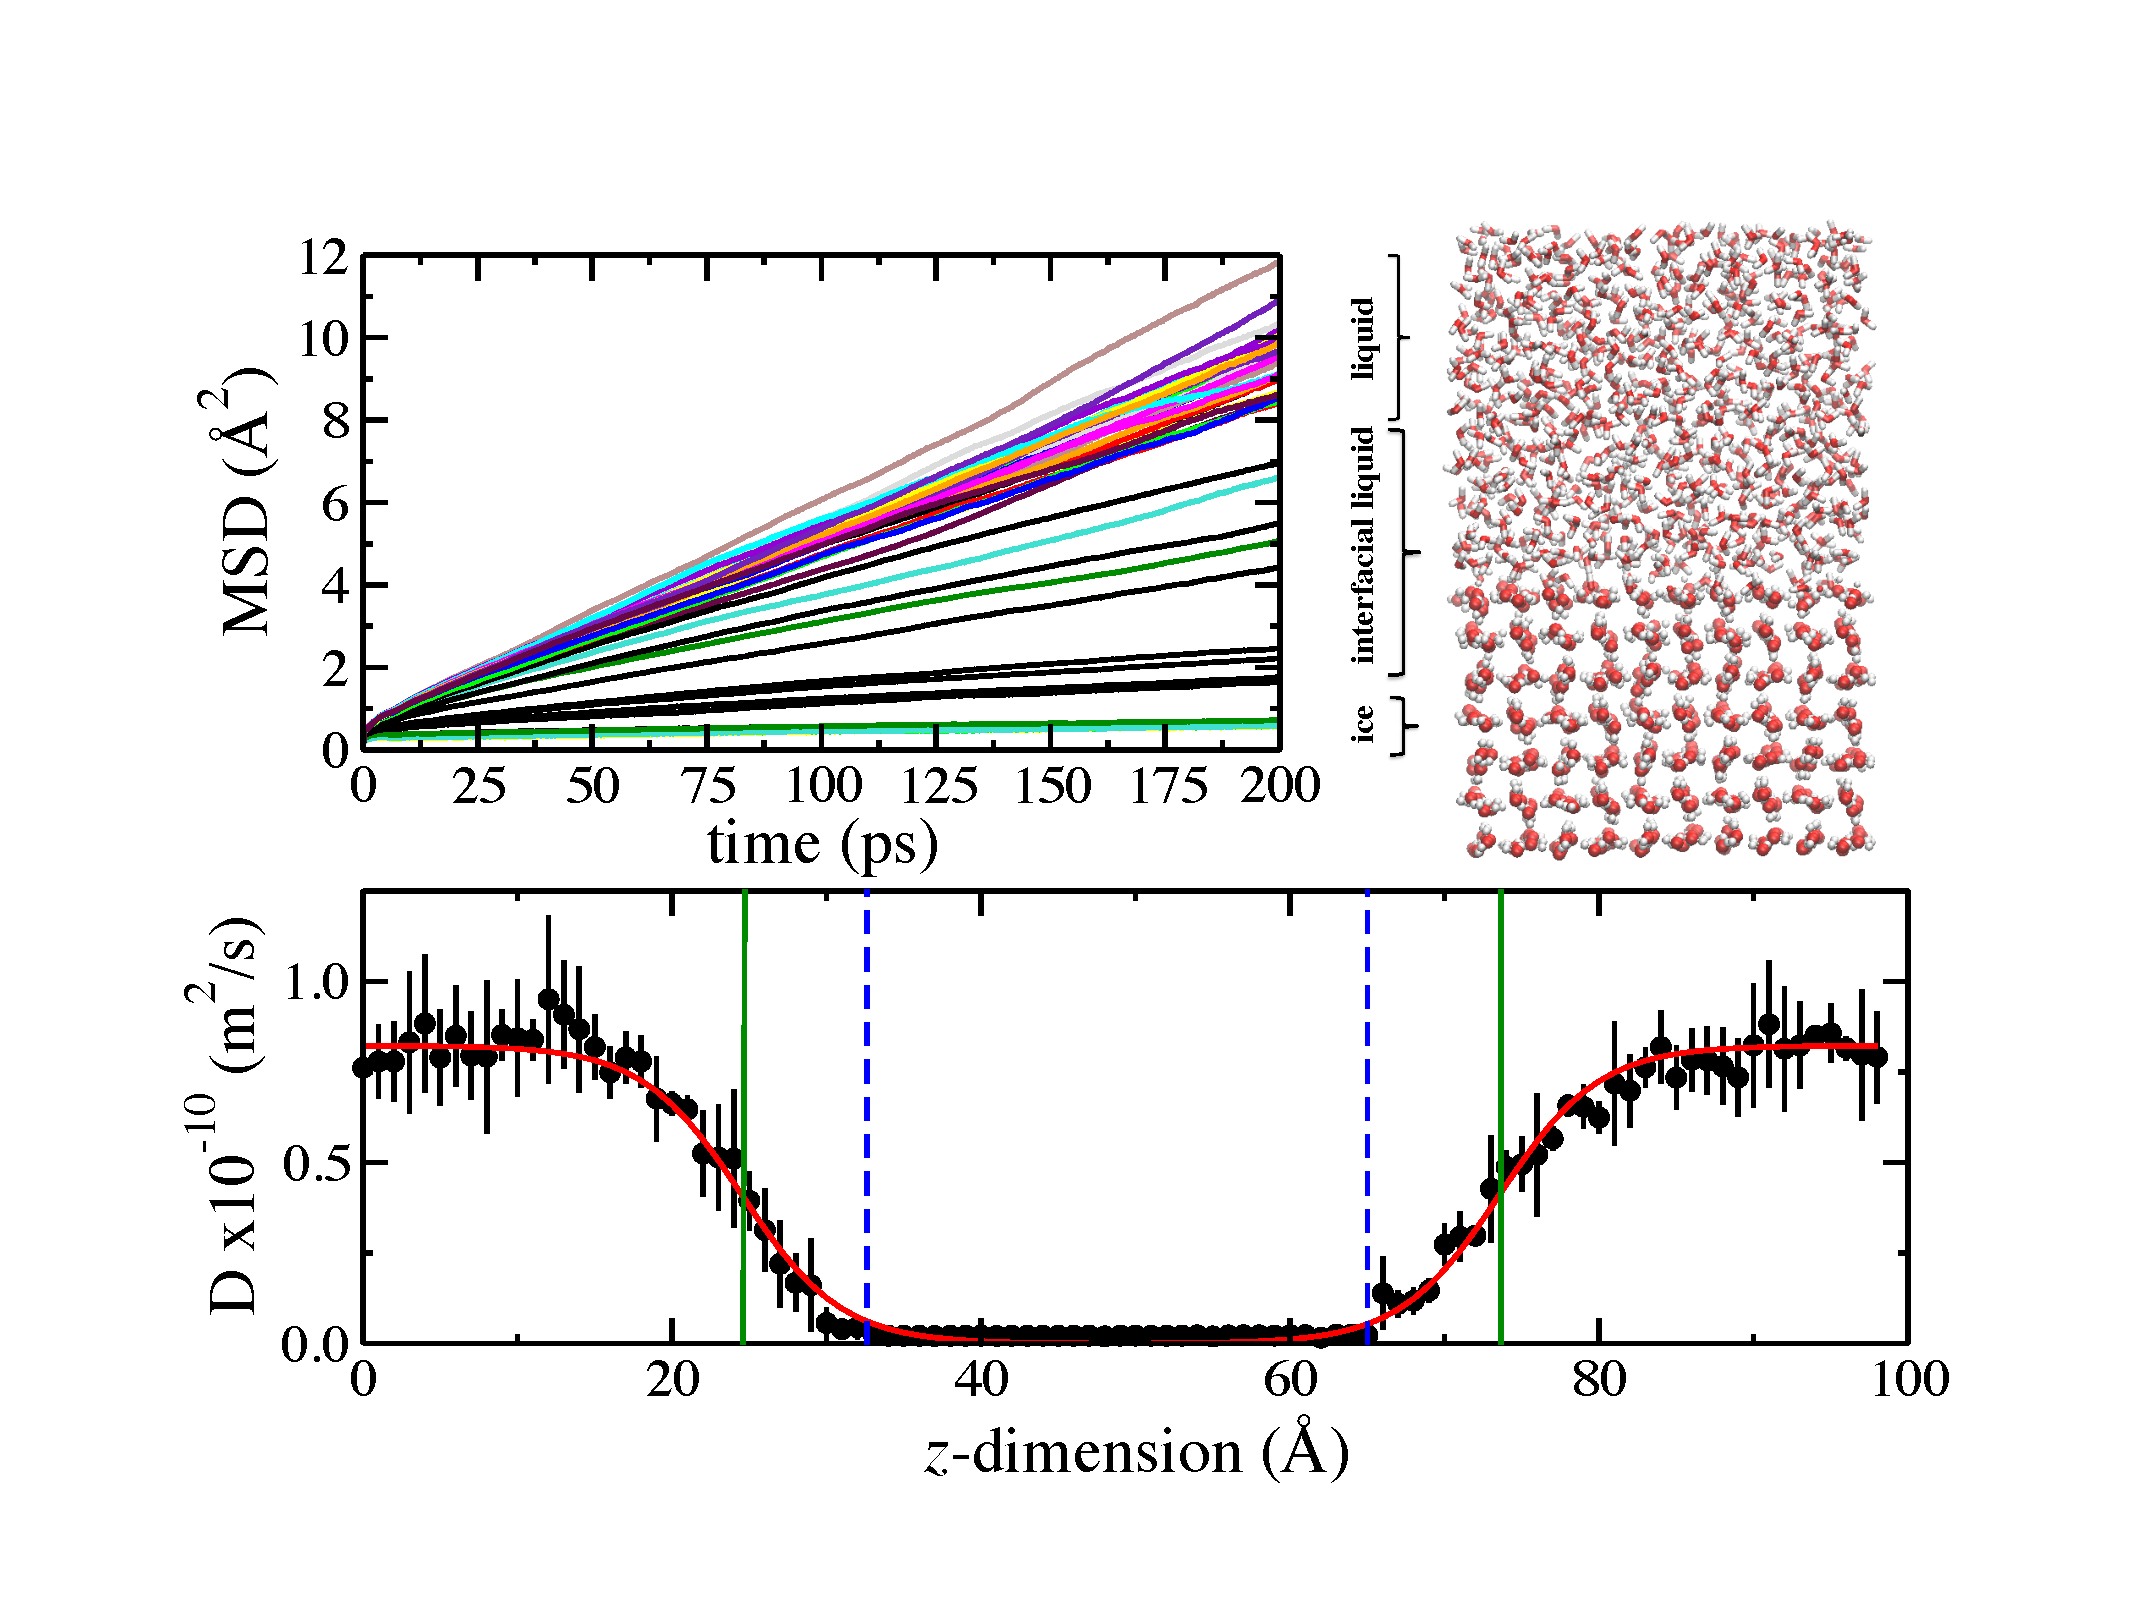
\includegraphics[width=\linewidth]{Figures/DzSPCE}
\caption{\label{fig:DzSPCE} Upper: Mean-squared displacement (MSD)
  collected in 1 \AA~bins across the SPC/E basal ice-I$_\mathrm{h}$ / water
  interface. The band with no increase in the mean-squared
  displacement are the water molecules in the ice, while the band
  increases most quickly corresponds to bins in the liquid. Between
  these two bands are bins which span the interfacial liquid water,
  with a mean-square displacement which increases moderately in
  time. Lower: The spatially resolved diffusion coefficient, $D(z)$,
  can be obtained from fitting the MSD data by
  Eq. \eqref{eq:diffusion3}. These are shown along with a fit that
  provies a ''diffusion'' width, $d_{10-90}^{D}$. The locations of
  the structural Gibbs dividing surfaces (using tetrahedrality) are
  indicated with vertical dashed blue lines, while the locations of
  the ''diffusion'' interfaces are shown in green.  }
\end{figure*}

\begin{figure*}
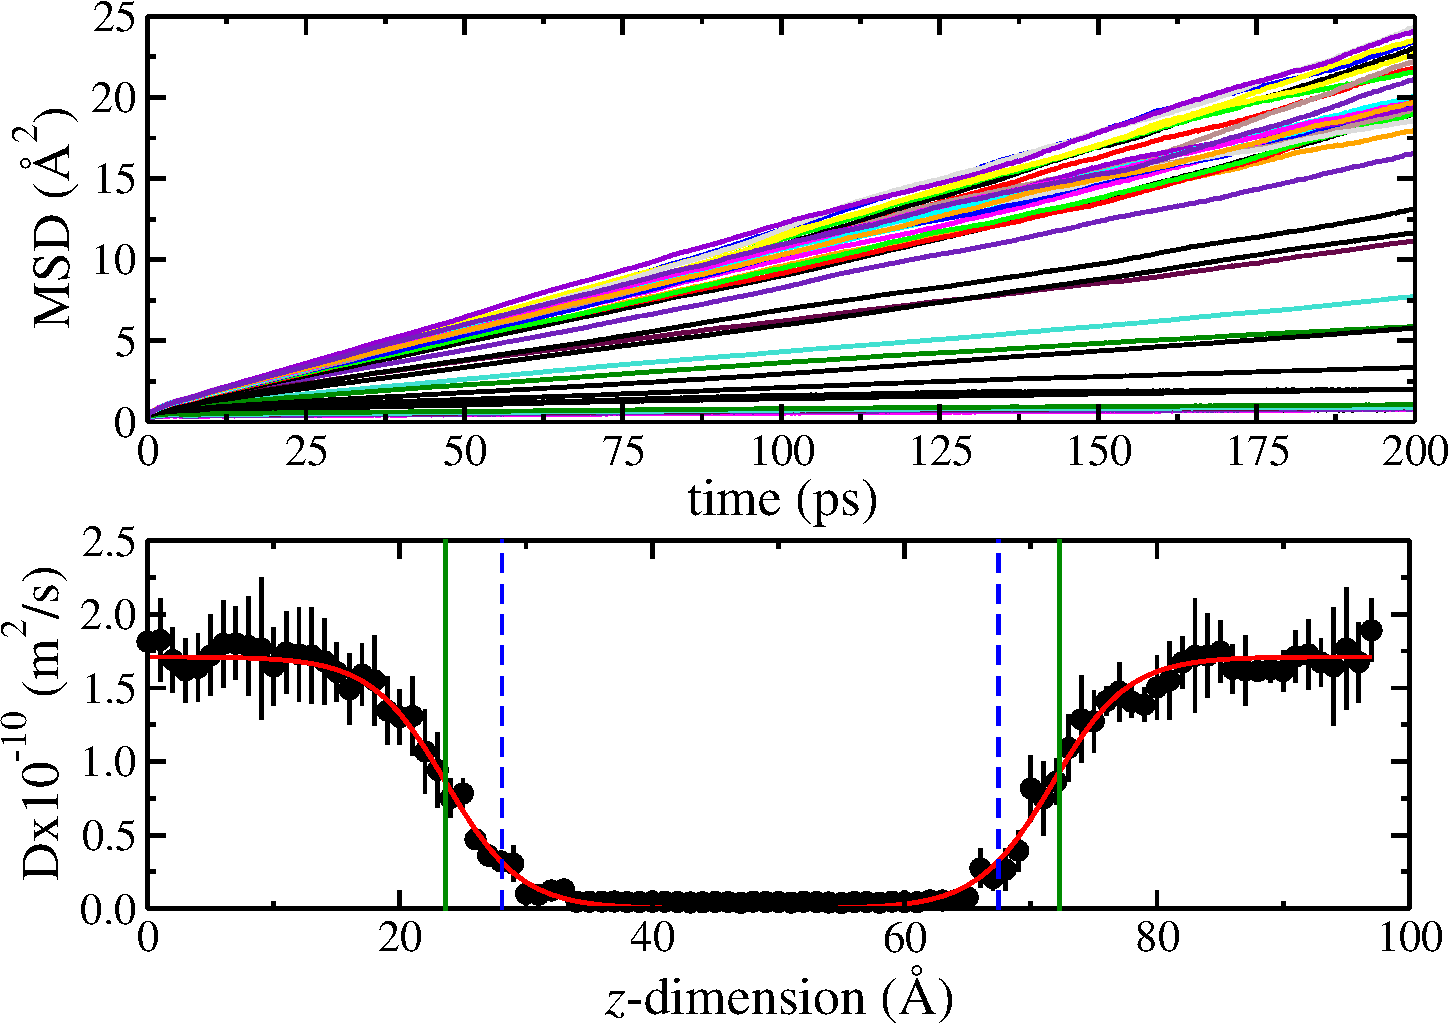
\includegraphics[width=\linewidth]{Figures/DzTIP4PIce}
\caption{\label{fig:DzTIP4PIce} The same basal diffusion coefficients
  as Fig. \ref{fig:DzSPCE}, but collected using the TIP4P/Ice model
  and at 270 K. Note that the higher coexistence temperature for this
  model increases the observed diffusion coefficients, and has brought
  the structural and diffusion interfaces much closer together.}
\end{figure*}

In the top panel of Figure \ref{fig:DzSPCE} and Figure
\ref{fig:DzTIP4PIce}, the mean-squared displacement
($\langle | \bm{r}_i(t) - \bm{r}_i(0) |^2 \rangle $) has been computed
for molecules within 1 \AA~bins across the basal ice-I$_\mathrm{h}$ /
water interface. At early times, the mean-square displacement rises
linearly due to ballistic motion of the molecules. This is due to the
unhindered motion of the water molecules within their local solvation
cages. At slightly longer times, the molecules bounce off of their
solvation cages, which can be seen in the short decay in the
mean-squared displacement immediately following the ballistic
regeime. Diffusion coefficients are obtained from a regression of the
longer time portion of the mean-squared displacements using
Eq. \eqref{eq:diffusion3}, and are shown in the lower panels of the
same figures. Calculation of the diffusion coefficients was performed
assuming the water molecules could translate in three dimensions, even
though it may be more appropriate to assume diffusion to occur in only
two dimensions for molecules close to the ice. 

In the bulk liquid portions of the SPC/E system (Figure
\ref{fig:DzSPCE}), diffusion coefficients are found to be XXX, while
in the ice the transport coefficient is numerically zero. In
comparison, diffusion constants for the liquid region of the systems
modeled with the TIP4P/Ice forcefield were found to be YYY. The
increase in the values reported is attributed to the warmer
temperature, 270~K. Fitting the $D(z)$ profiles with a function
designed to smoothly transition from the liquid diffusion coefficients
to those of the ice, we can determine the distance over which this
transition occurs.

\begin{equation}\label{eq:Dfit}
  D(z) = \frac{1}{D_\mathrm{liquid}} - \frac{1}{2D_\mathrm{liquid}} \left(
      \tanh \left( \frac{z-l}{d^D} \right) - \tanh \left( \frac{z-r}{d^D} \right) \right)
\end{equation}
  
Here, $D_\mathrm{liquid}$ is the value of the diffusion coefficient in
the liquid, $l$ and $r$ are the Gibbs dividing surface of the left and
right interfaces, and $d^{D}$ is the width of the interface. These
values of interfacial width are related to the structural $10\%-90\%$
interfacial widths reported in Chapter \ref{chap:Str} by the same
scaling coefficient, ($d_\mathrm{10-90}^{D} = 2.197~d^{D}$). All four
SPC/E interfaces exhibit dynamic widths that are $\sim~XX$~\AA~and are
larger than the structural measures reported in Table
\ref{tab:strWidths}. Similarly, the TIP4P/Ice systems at 270~K exhibit
dynamic widths of $\sim~YY$~\AA~, which are also larger than
interfacial widths predicted by structural measures for the same
model. As we saw with the structural measures of interfacial width,
the TIP4P/Ice model at 270~K predicts a broader interface than the
SPC/E model at 225~K.  The value of the dynamic width of the interface
for each interface is reported in Table \ref{tab:dynWidths}.

\begin{table}[h]
\centering
\caption{COMPUTED WIDTHS OF THE ICE-I$_\mathrm{h}$ / WATER INTERFACES BY
  DYNAMIC MEASURES. \label{tab:dynWidths}} 
\begin{tabular}{r|ccc|ccc}  
\hline
\hline
  \multirow{2}{*} & \multicolumn{3}{c|}{SPC/E (225~K)} &  \multicolumn{3}{c}{TIP4P/Ice (270~K) } \\
  & \multicolumn{3}{c|} {Interfacial Widths (\AA) \footnotemark[1]} &
                                                                      \multicolumn{3}{c} {Interfacial Widths  (\AA) \footnotemark[1]} \\
 Interface &  $d_\mathrm{10-90}^{D}$ & $d_\mathrm{10-90}^{C_2}$ &
                                                                  $d_\mathrm{10-90}^{jump}$  
                                                                 &
                     $d_\mathrm{10-90}^{D}$ & $d_\mathrm{10-90}^{C_2}$ & $d_\mathrm{10-90}^{jump}$\\ 
\hline
  Basal  $\{0001\}$                 & 14(4) & 11(2) & 12(2) & 13(2) & 15(3) & 11.1(8)  \\
  Prismatic  $\{10\bar{1}0\}$       & 15(3)  & 10(2) & 11(2) & 13(3) & 15(2) & 11(2)  \\
  14\degree~Pyramidal  $\{20\bar{2}1\}$   & 15(3) & 13(1) & 12(2) & 10(2) & 13(1) & 8.8(7)  \\
  Secondary Prism  $\{11\bar{2}0\}$ & 12(3) & 11(3) & 9(3) & 12(4) & 14(2) & 11(2)  \\ 
\hline
\hline
\end{tabular}
\flushleft
  \footnotemark[1]\footnotesize{Uncertainties in the last
   digit are indicated with parentheses.} \\
\end{table}

\section{Reorientation of Water Molecules}
The spatially-resolved orientational time correlation function,
\begin{equation}\label{C(t)1}
  C_{2}(z,t)=\langle P_{2}(\mathbf{u}_i(0)\cdot \mathbf{u}_i(t))
  \delta(z_i(0) - z) \rangle,
\end{equation}
provides local information about the decorrelation of molecular
orientations in time. Here, $P_{2}$ is the second-order Legendre
polynomial, and $\mathbf{u}_i$ is the molecular unit vector that bisects
the HOH angle of molecule $i$. The angle brackets indicate an average
over all the water molecules and time origins, and the delta function
restricts the average to specific regions in the $z$-dimension. 

In the ice crystal, decay of $C_2(z,t)$ is incomplete, while in the
liquid, correlation times are typically measured in ps. Observing the
spatial transition between the decay regimes can define a dynamic
measure of the interfacial width. To determine dynamic widths of the
interfaces under shear, each of the systems were divided into bins
along the $z$ axis ($\approx$ 1 \AA\ wide) and $C_2(z,t)$ was computed
using only those molecules that were in the bin at the initial
time. For each ice-I$_\mathrm{h}$ / water interface investigated, the following 0.5
ns simulations were computed: quiescent simulations (where no thermal
or momentum gradient was present), simulations with only a thermal
gradient present, and simulations where both thermal and momentum
gradients were present. During these simulations, the positions and
orientations of each molecule were recorded every 100 fs.

\begin{figure*}
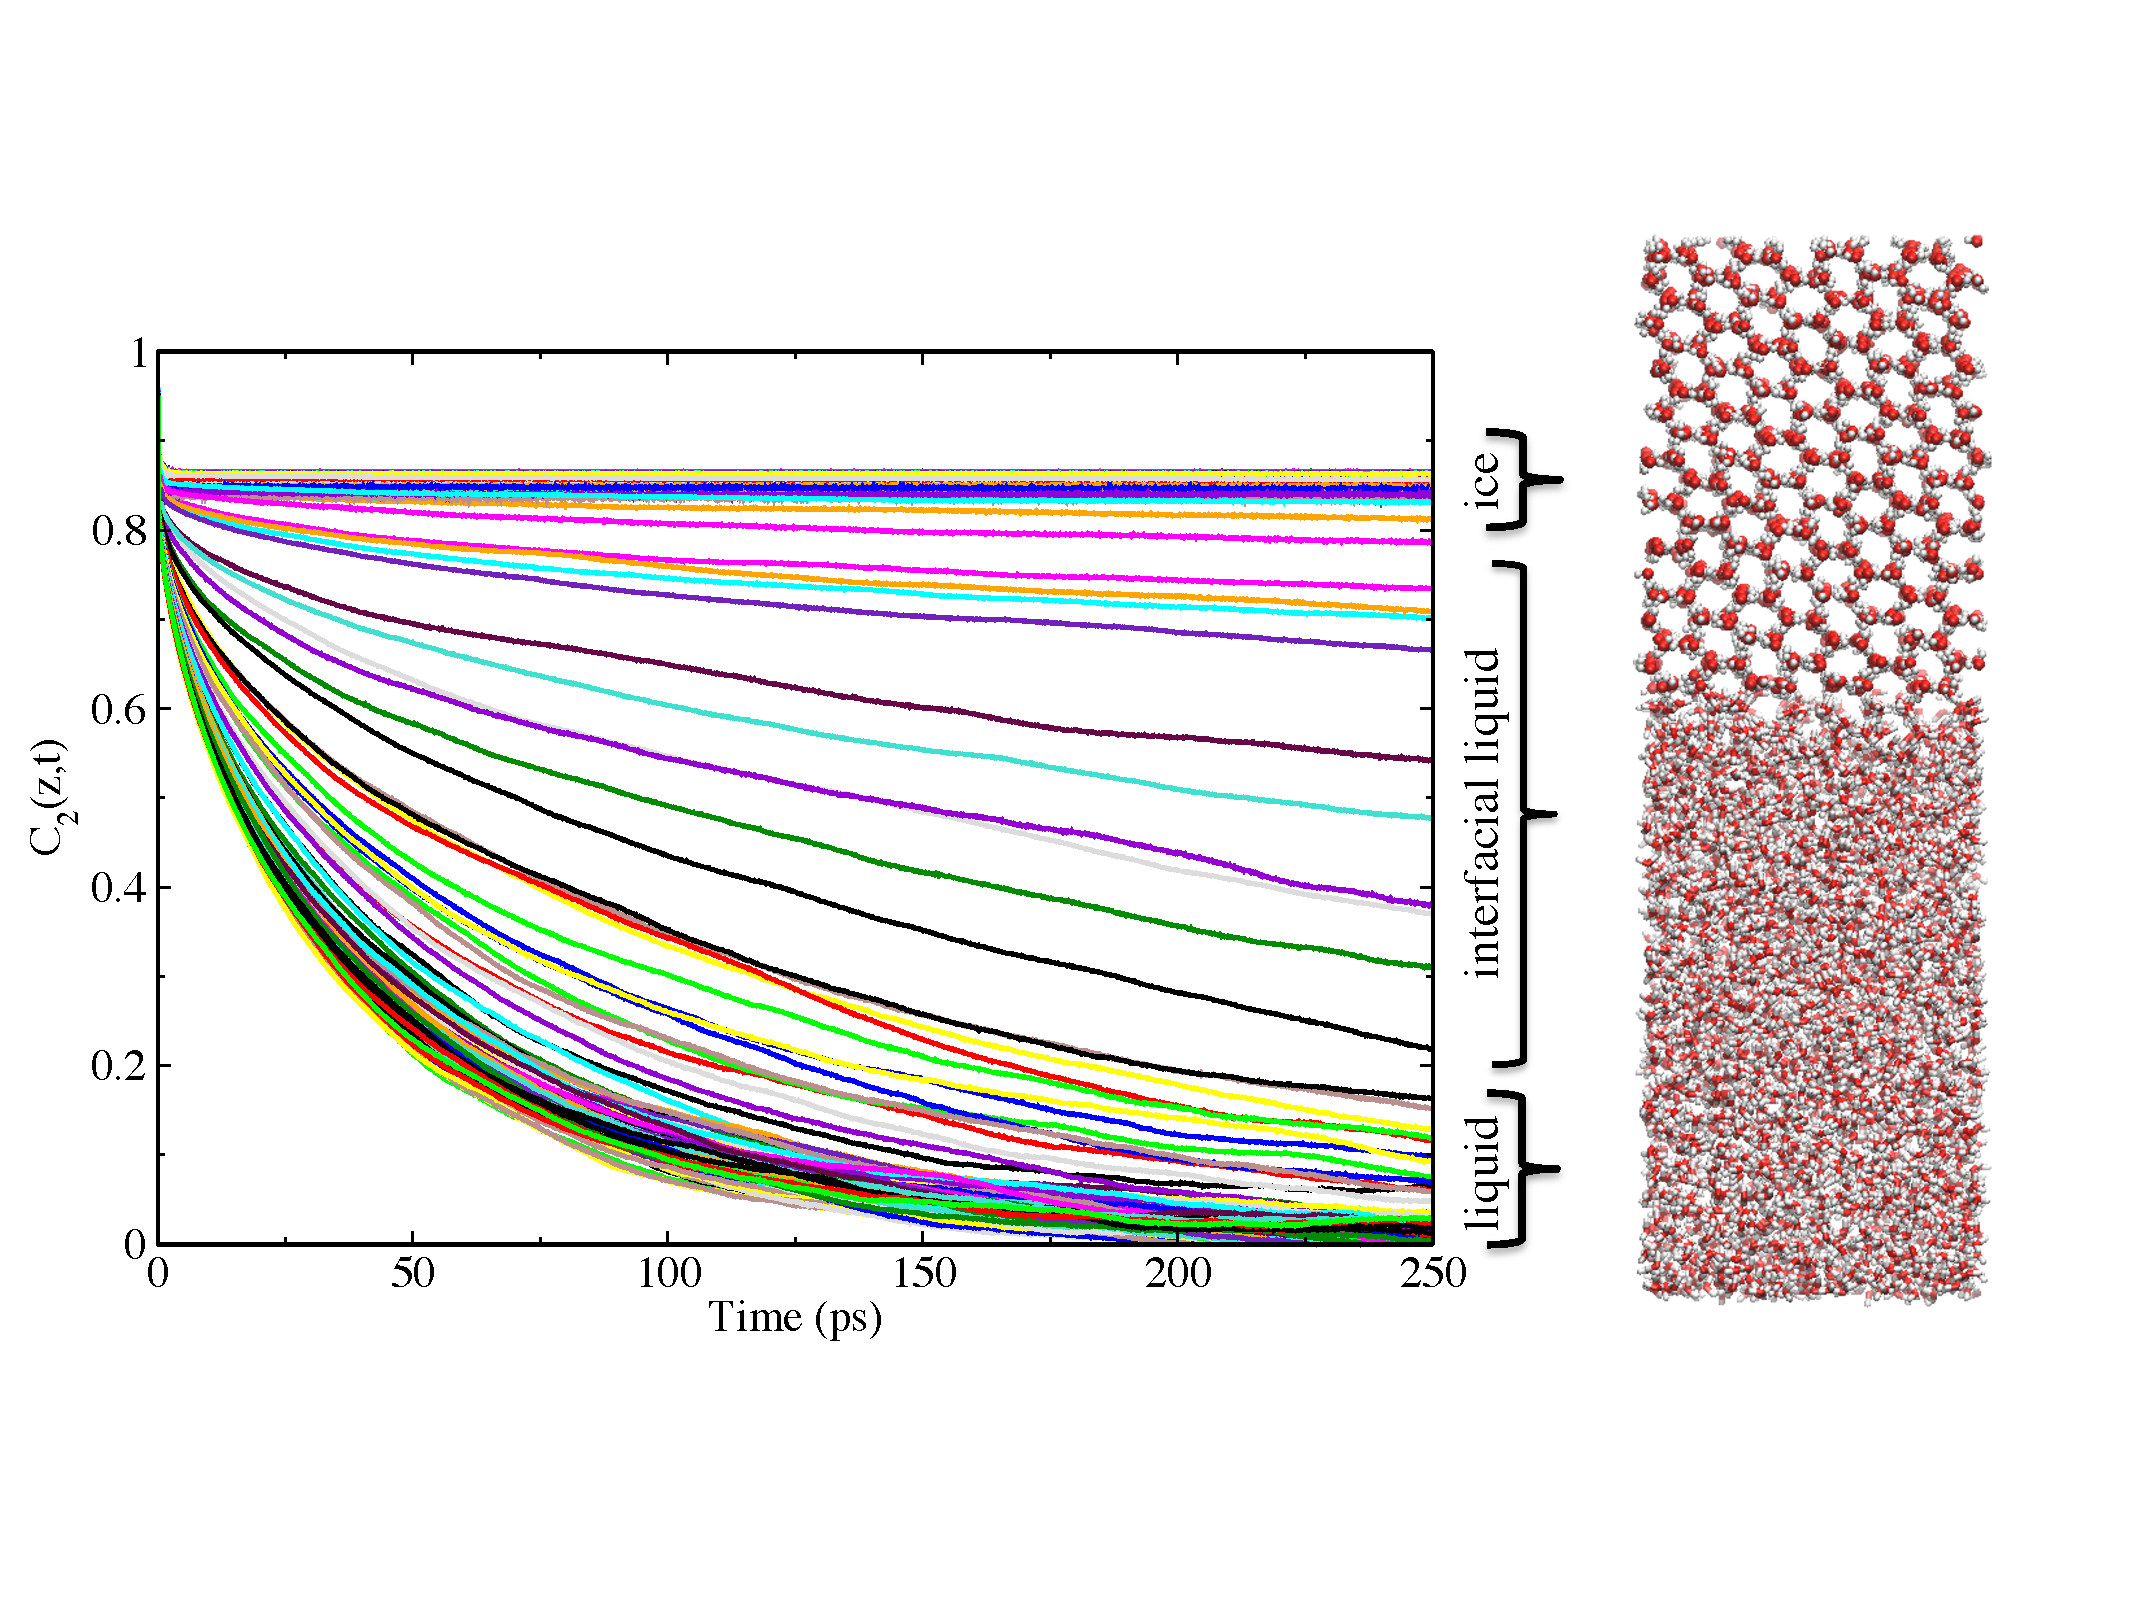
\includegraphics[width=\linewidth]{Figures/CztImage}
\caption{\label{fig:Czt} $C_2(z,t)$ collected in 1 \AA~bins across the SPC/E
  secondary prism ice-I$_\mathrm{h}$ / water interface. The band that experiences very
  little decay represents water molecules in the ice, while the band
  that decays quickly corresponds to bins in the liquid.  The
  correlation function presents a continuous distribution of decay
  behaviors across the interface between ice and liquid water.}
\end{figure*}

Recently, Laage and Hynes have determined the mechanism for water
reorientation.\cite{Laage2006,Laage2008} Using molecular dynamics
simulations, they found that water reorients by breaking a hydrogen
bond with an overcoordinated first-shell neighbor, and makes a large
angle jump to form a new hydrogen bond with an undercoordinated
second-shell neighbor. The hydrogen bond cleavage and molecular
reorientation occur in a concerted fashion, not in successive steps as
was previously thought. With this detailed picture, they constructed
the Extended Jump Model\cite{Laage2006,Laage2008} based on the Ivanov
Jump Model and parameters extracted from their molecular simulations;
the average jump amplitude of the rotational jump, $\theta_{0}$, and
the frequency of the jumps, $1/\tau_{0}$. After accounting for
molecular frame reorientation, the Extended Jump Model is able to
predict reorientation relaxation times, $\tau_{n}^{jump}$, which agree
with experimental results as well as estimates obtained from
simulations where fast librational motion is ignored.

Computed $C_2(z,t)$ values have previously been fit to a
triexponential decay, with three time constants:
$\tau_\mathrm{short}$, measuring the librational motion of the water
molecules, $\tau_\mathrm{middle}$, measuring the timescale for the
large angle jumps during the breaking and making of hydrogen bonds,
and $\tau_\mathrm{long}$, corresponding to the translational motion of
the water molecules.\cite{Louden2013a} The Extended Jump Model also
includes three similar decay constants, however two of them are linked
and the dynamics of the decay is governed by two parameters. Since we
are interested in how the decay times and the individual contributions
may change through the interface, we have fit the $C_2(z,t)$ data
with
\begin{equation}
  C_{2}(z,t) = a~e^{-t/\tau_\mathrm{short}} + b~e^{-t/\tau_\mathrm{middle}} + 
  (1-a-b)~e^{-t/\tau_\mathrm{long}}
\label{eq:c2}
\end{equation}
where all of the decay constants are considered local functions of the
$z$ coordinate. In Fig. \ref{fig:SPorient}, the $z$-coordinate
profiles for the three decay constants, $\tau_{\mathrm{short}}$,
$\tau_{\mathrm{middle}}$, and $\tau_{\mathrm{long}}$ for the secondary prism interface
is shown, along with their fractional components of the overall total
decay, ($a$, $b$, $1-a-b$), respectively. Similar figures for the
other interfaces are provided in the Supporting Information.

In the liquid regions of all four interfaces, $\tau_\mathrm{middle}$
and $\tau_\mathrm{long}$ consistently approach $3-6$ ps and $30-40$
ps, respectively.  Both of these times increase closer to the
interface.  Conversely, $\tau_\mathrm{short}$ decreases from a
liquid-state value of $72-76$ fs approaching the interface.

The fractional contributions of the three motions to the overall decay
changes as we approach the interface as well. Far from the ice, the
librational motion and hydrogen bond breaking/making events each
contribute to about 20 percent of the total decay, whereas frame
reorientation contributes about 60 percent. As we approach the
interface, the librations and hydrogen bond dynamics both decrease in
contribution. The librations comprise approximately 15 percent of the
overall decay at the edge of the interface, whereas the hydrogen bond
contributions drop to approximately zero. In contrast, the fraction of
the total decay due to frame reorientation is shown to increase
approaching the interface.  The time constant corresponding to this
motion is seen to logarithmically increase as we approach the interface
as the molecules become more ice-like. In the ice we would expect
molecular reorientation to be incomplete, however, at the interface we
observe frame reorientation to contribute 85 percent of the overall
decay.


\begin{figure*}
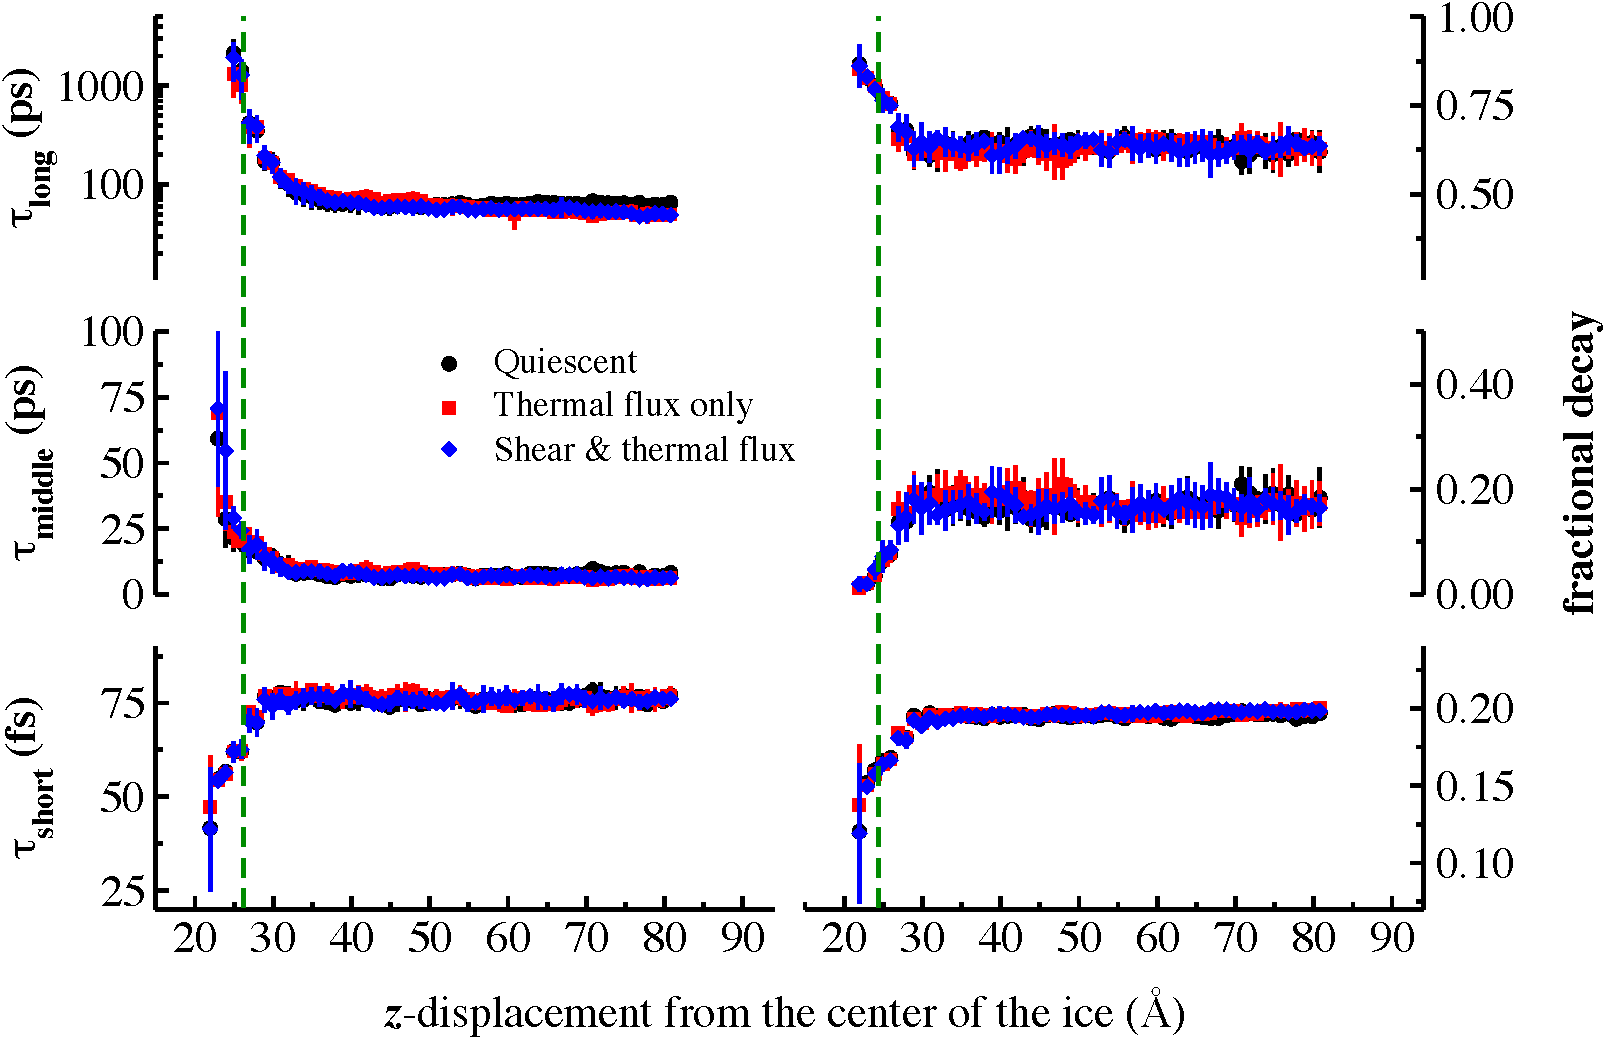
\includegraphics[width=\linewidth]{Figures/Sec_lcorrz}
\caption{\label{fig:SPorient} Decay times (left) for $C_2(z,t)$ at the
  SPC/E secondary prism interface, and their fractional contributions to the
  overall decay (right) fit using Eq. \eqref{eq:c2}. The local decay
  constants are plotted as a function of distance from the center of
  the ice slab. The vertical dashed line indicates the Gibbs dividing
  surface determined using the local tetrahedral order parameter.
  Results are shown for a quiescent system with no applied kinetic or
  momentum flux (black), an interface with an imposed
  kinetic energy flux (red), and a sheared simulation (blue) with both
  kinetic and momentum fluxes.}
\end{figure*}

The middle and long decay times diverge inside the ice crystal, so the
orientational rate, $k(z) = 1 / \tau(z)$ can be used to identify a
dynamic interfacial width for the interface by fitting the profiles of
the middle and long-time orientational rates with a function that goes
smoothly between bulk-like liquid behavior and the crystal,
\begin{equation}\label{tauFit}
  k(z) = \frac{1}{\tau_\mathrm{liquid}} - \frac{1}{2~\tau_\mathrm{liquid}} \left(
      \tanh \left( \frac{z-l}{d^{C_2}} \right) - \tanh \left( \frac{z-r}{d^{C_2}} \right) \right)
\end{equation}
where $l$ and $r$ are the locations of the Gibbs dividing surfaces,
and $d^{C_2}$ is a dynamic width.  As with the structural widths,
$10\%-90\%$ dynamic widths are easily computed from the fits
($d_\mathrm{10-90}^{C_2} = 2.197~d^{C_2}$), and are provided in Table
\ref{tab:dynWidths}. All four SPC/E interfaces exhibit dynamic widths
that are $\sim 11$~\AA, and are larger than the structural widths
computed above.  In TIP4P/Ice at 270K, the dynamic widths are
$\sim 14$~\AA, also larger than the structural widths in for these
interfaces.

We note that Bryk and Haymet also calculated the orientational time
correlation function at the basal interface of SPC/E
water,\cite{Bryk2002} and observed the same qualitative trend through
the ice-I$_\mathrm{h}$ / water interface, although the spatial resolution was not
sufficient to resolve a dynamic width.
 
\section{Spatial Resolution of Hydrogen Bond Jump Rates}
The spatially-resolved hydrogen bond jump correlation function,
\begin{equation}\label{jump}
C_\mathrm{jump}(z,t) = 1 - \langle n_a(0) n_b(t) \delta(z_i(0) - z) \rangle
\end{equation}
measures the decorrelation of a hydrogen bond on molecule $i$ as it
transitions between one acceptor ($a$) and another ($b$). $n_a(0)$ is
set to one if hydrogen $i$ is bound to acceptor $a$ at time $0$, and
is zero otherwise.  Absorbing boundaries are utilized with this
correlation function; switches from $b$ back to $a$ at a later time
are considered a new jump, and the angle brackets indicate an average
over all donor hydrogens and time origins. Laage and Hynes determined
the bulk version of this function had \textit{single}-exponential
decay in room temperature water.

A version of this correlation function was used to investigate how
water molecules reorient around
ions\cite{Laage2007,Laage2008a,Stirnemann2011a,Laage2011},
proteins\cite{Duboue-Dijon2014}, and in confined
spaces\cite{Laage2012b,Fogarty2014}.  Laage and Hynes studied how the
strength of the hydrogen bond might perturb the reorientation
dynamics,\cite{Laage2006a} and found the librational motion which
forms a cone around the O-O vector is smaller for more strongly
hydrogen bonded water. This may also provide a partial explanation for
the increasing contribution of short time orientational decay very
close to the ice surfaces.  Since the solid creates an excluded volume
for the water molecules that are in proximity to the interface, the
hindered range of motion (i.e., a smaller cone around the O-O vector)
manifests as faster librational decay.

As an additional measure of a dynamic width of the quiescent
interfaces, each of the systems were divided into bins along the $z$
axis ($\approx$ 1 \AA\ wide) and $C_\mathrm{jump}(z,t)$ was computed
(see Fig. \ref{fig:SPkjmp} and Fig. \ref{fig:SPTIP4Pkjmp}).
Like Laage and Hynes, we find that within each spatial region, the
decay is easily fit with a single exponential, yielding a local
hydrogen bond jump time. The jump times diverge inside the ice
crystal, so the jump rate, $k_\mathrm{jump}(z) = 1 / \tau_0(z)$ can be
used to identify a hydrogen bond jump width for the interface in a
similar manner to the dynamic width. $k_\mathrm{jump}(z)$ was fit with
a hyperbolic tangent (see Eq. \eqref{tauFit}) and the $10\%-90\%$ jump
width, $d_\mathrm{10-90}^{jump}$, is shown in Table \ref{tab:dynWidths}.

\begin{figure*}
\includegraphics[width=5.5in]{Figures/secPrismJumpPlot}
\caption{\label{fig:SPkjmp} Upper: Hydrogen bond jump correlation
  functions, $C_\mathrm{jump}(z,t)$, collected in 1 \AA~bins across
  the SPC/E secondary prism ice-I$_\mathrm{h}$ / water interface. The band that
  experiences very little decay represents water molecules in the ice,
  while the band that decays quickly corresponds to bins in the
  liquid.  The correlation function presents a continuous distribution
  of decay behaviors across the interface between ice and liquid
  water.  Lower: $C_\mathrm{jump}(z,t)$ decays exponentially, and each
  1 \AA~spatial bin can be fit with a jump rate, $k_\mathrm{jump}(z)$.
  These are shown with a fit that provides a ``jump'' width,
  $d_\mathrm{10-90}^{jump}$. The locations of the structural Gibbs dividing
  surfaces (using tetrahedrality) are indicated with vertical dashed
  blue lines, while the locations of the ``jump'' interfaces are shown in
  orange.}
\end{figure*}


\begin{figure*}
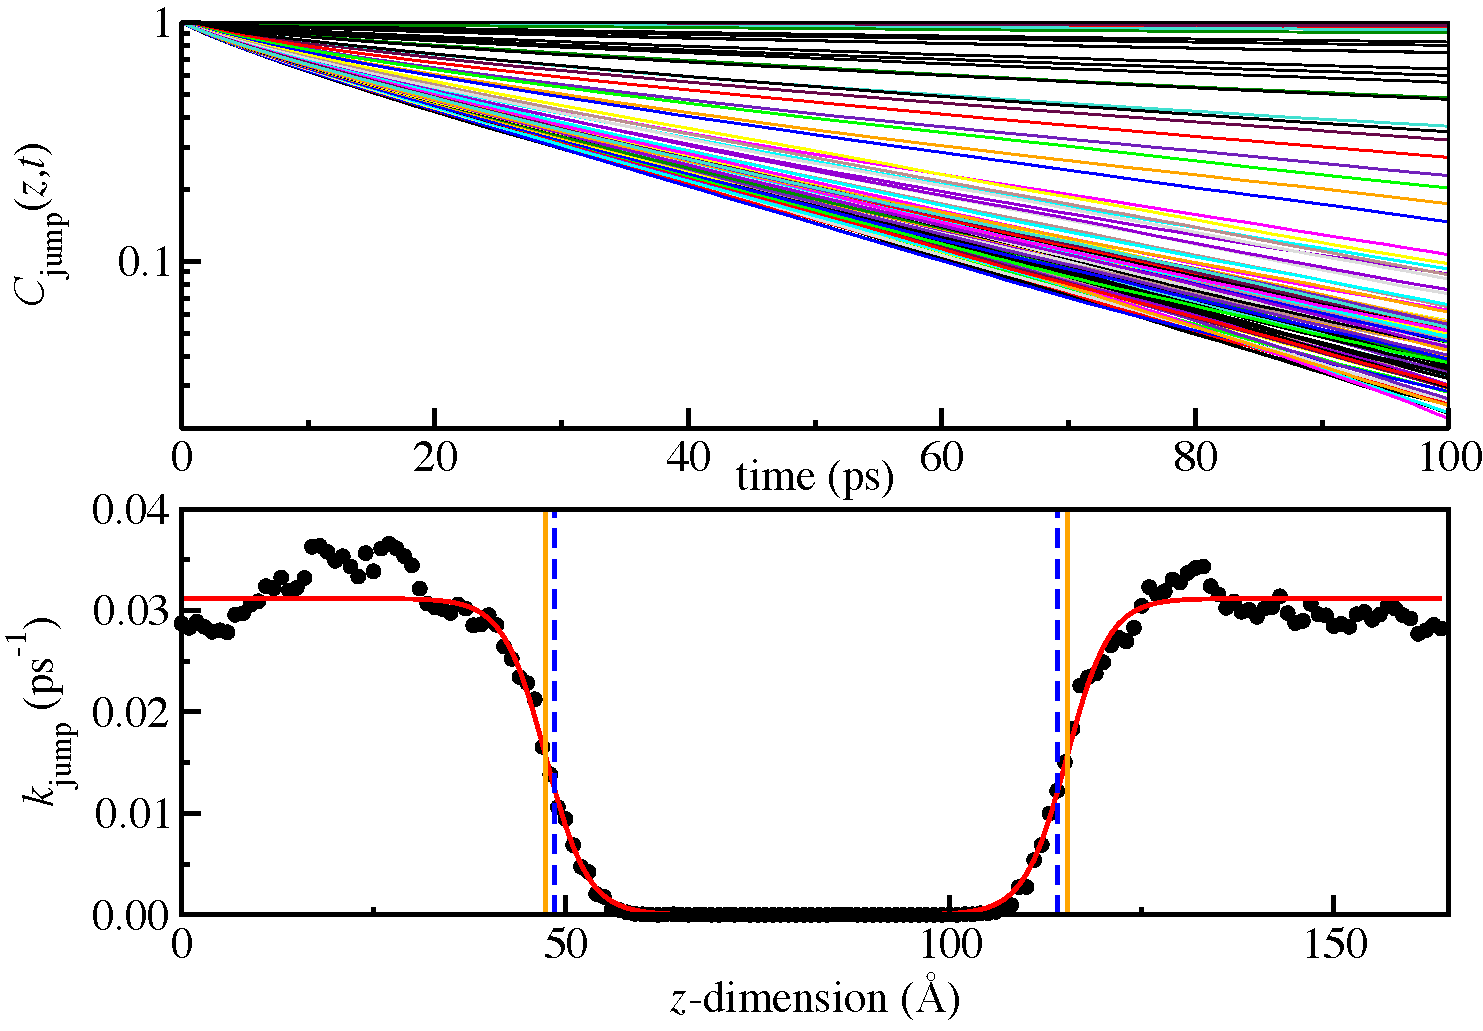
\includegraphics[width=\linewidth]{Figures/secprismJumpPlotTIP4PIce}
\caption{\label{fig:SPTIP4Pkjmp} The same secondary prism hydrogen
  bond jump data as Fig. \ref{fig:SPkjmp}, but collected using the
  TIP4P/Ice model and at 270~K.  Note that the higher coexistence
  temperature for this model increases the observed liquid-state jump
  rates, and has brought the structural and jump interfaces much
  closer together.}
\end{figure*}


\section{Summary}
In this chapter, we have presented dynamic ice-I$_\mathrm{h}$ / water
interfacial widths as evaluated by three separate order parameters. In
all three cases, the dynamic order parameters predicts a much broader
interfacial width than either of the structural analyses described in
Chapter \ref{chap:Str}.  For SPC/E ice-I$_\mathrm{h}$ / water
interfaces, the self diffusion coefficient gives an estimate of about
13 \AA~, while the TIP4P/Ice interface is found to be YYY \AA~. These
results agree well with other two order parameters investigated, the
orientational time correlation function, and the hydrogen bond jump
time. For each interface, the width predicted by the TIP4P/Ice model
is slightly broader than compared to the SPC/E model, namely due to
the warmer coexistence temperature. 
